\documentclass[tikz]{standalone}
\usepackage{tikz}
\usetikzlibrary{arrows.meta,positioning,shapes.geometric,shapes.misc,fit,backgrounds,calc,decorations.pathreplacing}

\begin{document}
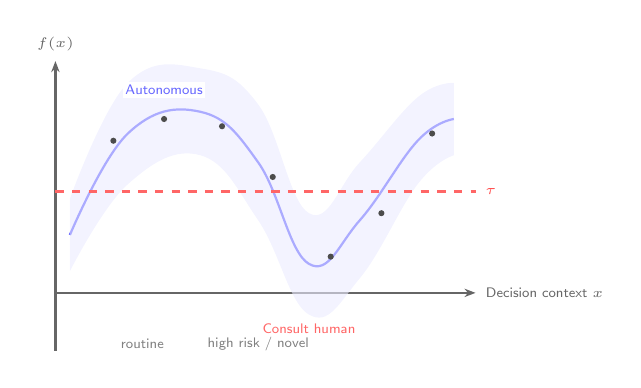
\begin{tikzpicture}[scale=0.92]
% Axes
\draw[-{Stealth[length=4pt]}, thick, black!60] (0,0) -- (5.8,0) node[right, font=\tiny\sffamily] {Decision context $x$};
\draw[-{Stealth[length=4pt]}, thick, black!60] (0,-0.8) -- (0,3.2) node[above, font=\tiny\sffamily] {$f(x)$};

% GP mean curve
\draw[thick, blue!70] plot[smooth, tension=0.7] coordinates {(0.2,0.8) (1,2.2) (2,2.5) (2.8,1.8) (3.5,0.4) (4.2,1.0) (5,2.1) (5.5,2.4)};

% Confidence band
\fill[blue!8, opacity=0.6] plot[smooth, tension=0.7] coordinates {(0.2,0.3) (1,1.5) (2,1.9) (2.8,1.0) (3.5,-0.3) (4.2,0.2) (5,1.5) (5.5,1.9)} -- plot[smooth, tension=0.7] coordinates {(5.5,2.9) (5,2.7) (4.2,1.8) (3.5,1.1) (2.8,2.6) (2,3.1) (1,2.9) (0.2,1.3)} -- cycle;

% Threshold line
\draw[dashed, red!60, thick] (0, 1.4) -- (5.8, 1.4);
\node[font=\tiny\sffamily, text=red!70, anchor=west] at (5.8, 1.4) {$\tau$};

% Autonomous zone
\node[font=\tiny\sffamily, text=blue!60, fill=white, inner sep=1pt] at (1.5, 2.8) {Autonomous};

% Human zone
\node[font=\tiny\sffamily, text=red!60, fill=white, inner sep=1pt] at (3.5, -0.5) {Consult human};

% Observation points
\foreach \x/\y in {0.8/2.1, 1.5/2.4, 2.3/2.3, 3.0/1.6, 3.8/0.5, 4.5/1.1, 5.2/2.2} {
    \fill[black!70] (\x, \y) circle (1.2pt);
}

% Labels
\node[font=\tiny\sffamily, text=black!50] at (2.8, -0.7) {high risk / novel};
\node[font=\tiny\sffamily, text=black!50] at (1.2, -0.7) {routine};

\end{tikzpicture}
\end{document}
